\subsubsection{Search Space}

Bei der Optimierung einer Anfrage geht es um die Entscheidung, welches der optimale Plan für eine Anfrage ist. Um diese Entscheidung zu treffen, müssen mehrere Alternativen gegeben sein, zwischen denen an Hand von Entscheidungskriterien der optimale Plan gefunden werden kann. Die Suche nach Entscheidungsalternativen spielt eine entscheidende Rolle bei der Anfragenoptimierung.


\begin{figure}[h]
  \centering
  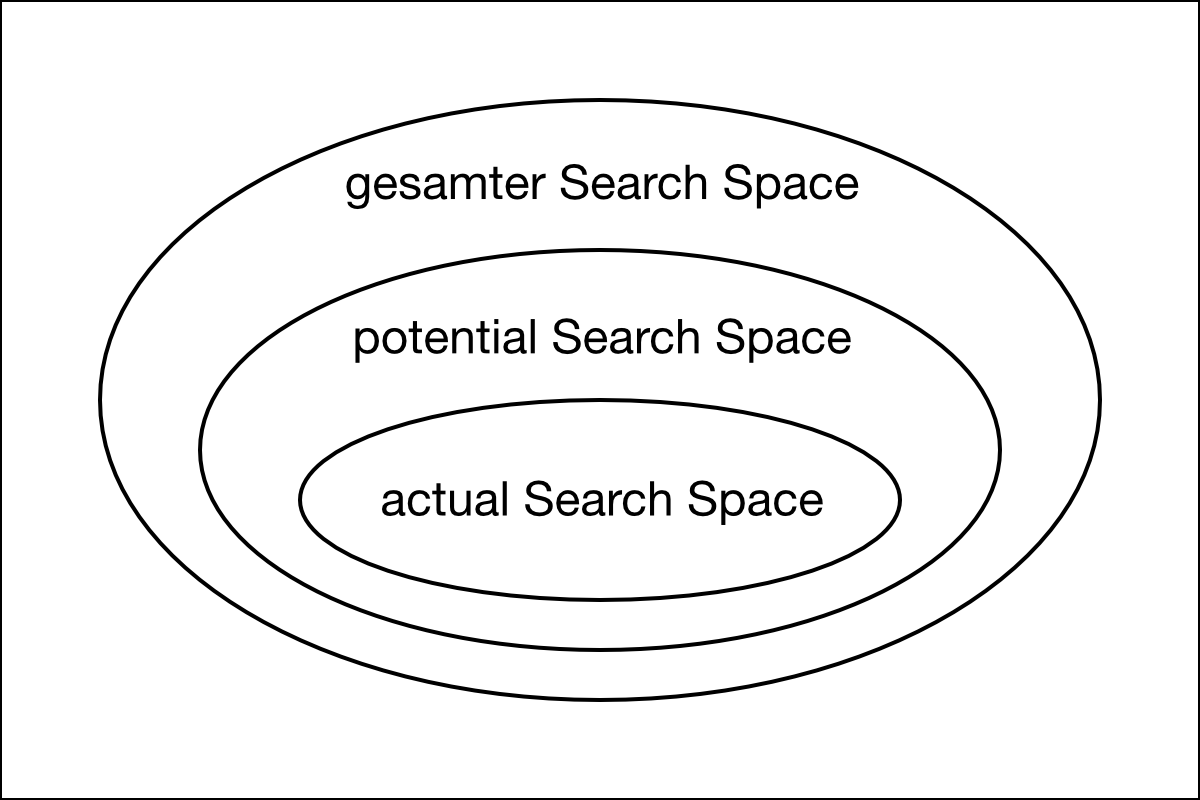
\includegraphics[width=\textwidth]{02_Grundlagen/SearchSpace.png}
  \caption{Search Space}
  \label{SearchSpace}
\end{figure}

Für die Anfragenoptimierung ist es notwendig, dass eine Menge logisch äquivalenter Pläne gefunden wird. Die Menge der logisch äquivalenten Pläne wird als Search Space oder Suchraum bezeichnet. Er beinhaltet alle Pläne, die aus einer Anfrage gebildet werden könnten. Die Menge aller möglichen Pläne kann sehr gross sein und nicht jeder Plan mit gängigen Mitteln gefunden werden. Die Pläne, die nicht mit gängigen Mitteln erreicht werden können, werden als nicht erreichbar bzw. non-accessable bezeichnet. Pläne die durch eine Technik hingegen erreicht werden können, heissen potenzieller Suchraum (Potential Search Space). Innerhalb dieses Raums finden sich alle Pläne, die durch technische Mittel erzeugt werden können und somit erreichbar bzw. accessable sind.  Da selbst die Menge der Pläne im potential Search Space sehr hoch sein kann, beschränken sich Optimierer i.d.R. auf ein Subset von Plänen und brechen die Suche irgendwann ab. Der Suchraum, der tatsächlich erforscht wurde und durch den Optimierer gebildet wurde, wird als tatsächlicher oder actual Search Space bezeichnet.


Wie in Abbildung \ref{SearchSpace} zu sehen, ist es ideal, wenn der actual Search Space Teil des potential Search Spaces und der potential Search Space auch weit des Search Spaces ist. Dies ist jedoch nicht immer der Fall. Anfragenoptimierer können auch fehlerhafte, nicht äquivalente, Pläne erzeugen, die fälschlicherweise dem actual Search Space zugeordnet sind.

Die Erforschung eines Suchraums kann beispielsweise mit Hilfe von regelbasierten Transformatoren geschehen. Sie verwenden Regeln um aus einem Ausgangsplan einen anderen Plan zu erzeugen. Das Ergebnis, die Menge aller erforschten Pläne dient der Kostenschätzung als Grundlage zur Berechnung der Kosten. Die eigentliche Auswahl geschieht durch Enumeratoren, die den günstigsten Plan in der Menge des actual Search Spaces ausfindig machen.






